% This is the section of the results focused on the assembly


\section{Transcriptome Assembly}

\subsection{Assembly Quality}
\subsubsection{Quality Statistics}
\subsubsection{Example Transcripts}
To assess the data/assembly quality further, I used canonical transcripts of \textit{C. acetobutylicum}, to understand the agreement of the coverage, the assembly, and the existing annotation. Six issues, listed below, were considered for each example to better understand the quality of the assembly and the degree of curation required. 
\begin{enumerate}
\item Is the transcript large enough to include the known ORFs and RBSes?
\item Does the assembled transcript's TSS agree with promoter motifs?
\item Does it agree with published transcription start sites?
\item Does the assembled transcript's size agree with published Northern blots?
\item Does the assembly represent the coverage and if not, which of these two best represents the biological knowledge of this region?
\item Does the assembled region require curation (e.g. fused, extended, or truncated transcripts)?
\end{enumerate}
Agreement between the data and the literature would support the efficacy of this technique. Its effectiveness is particulary important in cases where no previous experimental data exists. These results could be very useful to future studies if only minimal remediation or curation is required. The first example that I examine is the Sol locus.

The Sol locus is a 5.1kb region (basepairs 175,530-180,650) on the pSol1 megaplasmid that is responsible for the production of several solvents. This region encodes several enzymes including a tri-functional NAD(H\textsuperscript{+})-dependent alcohol/aldehyde dehydrogenase, two coenzyme-A transferases, and an acetoacetate decarboxylase. The region is also home to a protein SolR, which includes a helix-turn-helix motif and is thought to regulate solventogenesis. These genes are vital for acid reuptake and conversion into alcohols, a vital part of this organism's metabolism and the solventogenesis process.


In this dataset, we observe strong coverage of the Sol operon, SolR, and Adc. The Sol operon has continuous coverage(\textgreater 10,000x) across the entire 4.1kb transcript. The Adc gene has a comparable coverage pattern, representing 0.8kb monocistronic transcript. The regulatory protein SolR has a lower degree of coverage (\textgreater 300x) across its 1.1kb transcript. All transcript sizes agree with Northern blots of this locus in the literature.
%          SOL LOCUS Fig 1.
\begin{figure}
\small
{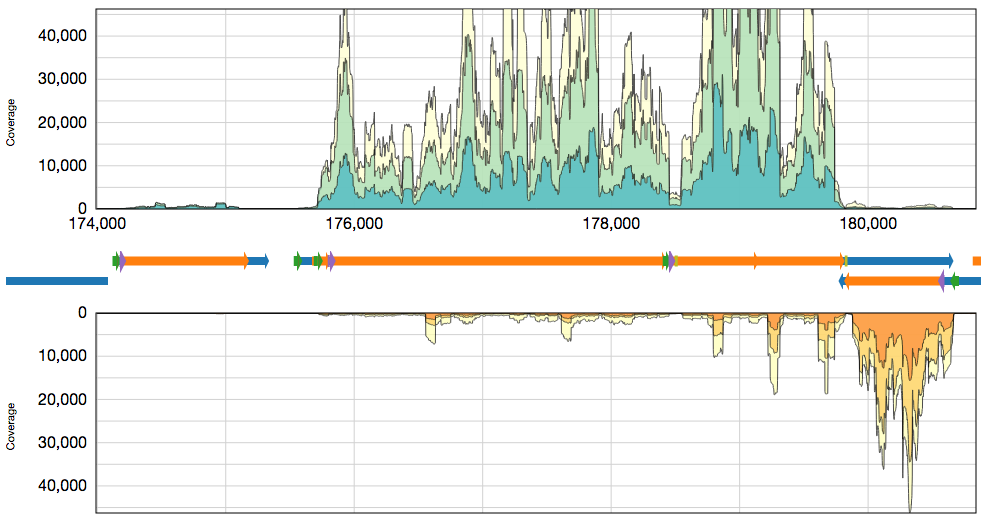
\includegraphics[width=\textwidth,height=2.5in]{images/Assembly/Sol/Sol-locus.png}
\subcaption{Sol locus}\label{fig:1a}}
% \label{fig:1}
\caption{Sol Locus: The Sol operon (\subref{fig:1a}) upper track) consists of OrfL, alcohol dehydrogenase (AdhE), and Co-A transferases A and B (ctfA,ctfB). SolR (far left) and acetoacetate decarboxylase (ADC; \subref{fig:1a} lower track, right) are also shown. Coverage for the Watson and Crick strands (top and bottom tracks) are visualized with an annotation track (center). Tracks show cumulative coverage for unstressed (yellow), butanol (light green/ light orange), and butyrate (green/orange) stressed samples over all time points. Transcripts (blue), ORFs (orange), RBSes (purple), inverted repeats (yellow), promoters (green), and TSSes (red) are represented as arrows and bars.}
\end{figure}
The assembly suggests a distal transcription start site for the Sol operon at 175,564, agreeing with two previous studies of this region. Several increases in coverage are observed just after the proximal promoter as well. It is understood that the proximal promoter is the most active promoter motif for the Sol operon and this view is supported by our data. The assembly also shows a distinct transcription start site for SolR, in agreement with previous findings. The coverage data also agree with the single transcription start site for Adc, shown as a distinct increase in coverage. However, the Adc transcript has been misassembled, fused to residual signal upstream of the true TSS. This is the first example of misassembly, which I address in the next section.
% Transcription start sites SOL Fig 2.
\begin{figure}
\small
{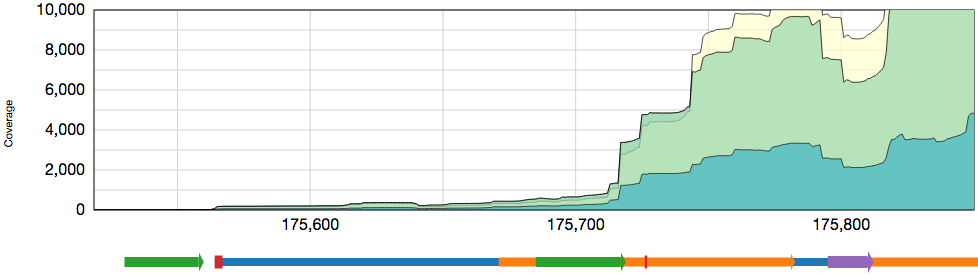
\includegraphics[width=\textwidth,height=1.5in]{images/Assembly/Sol/Sol-TSS.png}
\subcaption{Sol operon transcription initiation region}\label{fig:2a}}
{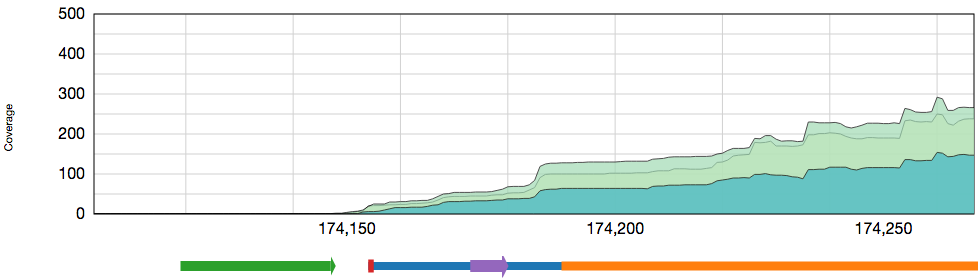
\includegraphics[width=\textwidth,height=1.5in]{images/Assembly/Sol/Sol-SolR-TSS.png}
\subcaption{SolR transcription initiation region}\label{fig:2b}}
{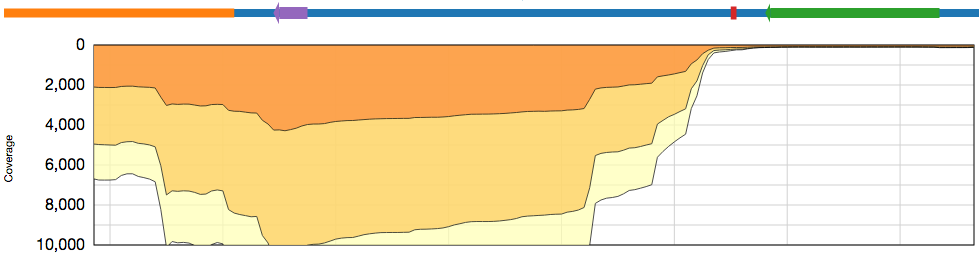
\includegraphics[width=\textwidth,height=1.5in]{images/Assembly/Sol/Sol-Adc-TSS.png}
\subcaption{Adc transcription initiation region}\label{fig:2c}}
%\label{fig:1.5}
\caption{Sol Locus Transcription Start Sites: \subref{fig:2a}) Sol operon (OrfL, AdhE) transcription start sites. The coverage and assembly data have strong agreement with previously described proximal and distal promoters and transcription start sites. \subref{fig:2b}) The assembled transcription start site for SolR agrees with previous findings. \subref{fig:2c}) Transcription initiation region for Adc. While the coverage clearly shows the appropriate increase, the transcription start site has been fused to residual coverage upstream of the true TSS. }
\end{figure}
\begin{figure}
{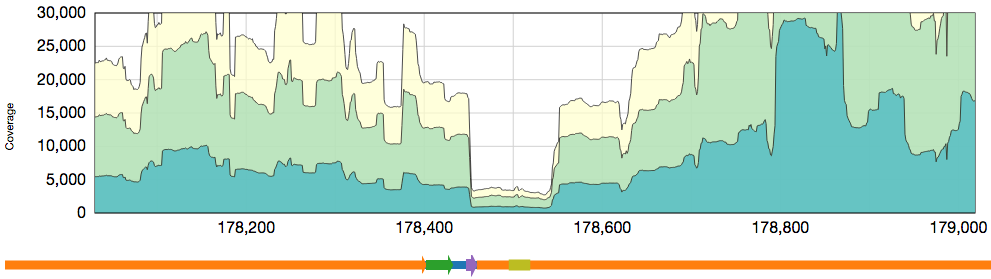
\includegraphics[width=\textwidth,height=1.5in]{images/Assembly/Sol/Sol-AdhE-terminator.png}
\subcaption{Putative AdhE terminator, CtfA/B promoter}\label{fig:3a}}
{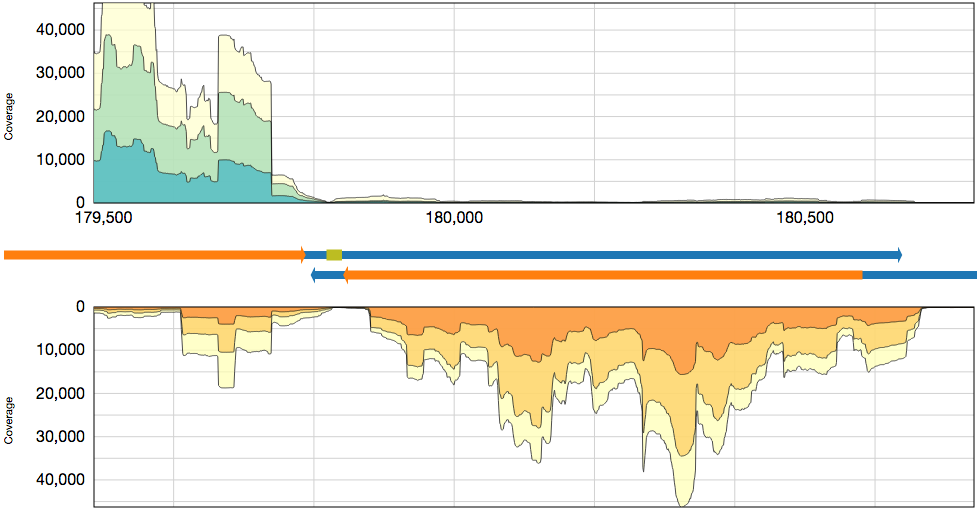
\includegraphics[width=\textwidth,height=2.5in]{images/Assembly/Sol/Sol-bifunctional-terminator}
\subcaption{Bifunctional Rho-independent terminator for Sol operon, Adc}\label{fig:3b}}
\caption{Sol Locus Transcription Stop Sites: \subref{fig:3a}) Low coverage in the Sol operon. A terminator may be partially responsible for a sustained low coverage level in the Sol operon. Additionally, a promoter motif was located upstream of the CtfA RBS and the pattern of expression is consistent with the beginning of a new transcript. \subref{fig:3b}) A bifunctional terminator, likely responsible for transcriptional termination of both Adc and the Sol operon. }
\end{figure}

The depth of coverage is also fairly consistent across these regions, except for a ~100bp region near the N-terminus of CtfA. This decrease in coverage can be explained by an inverted repeat present in this region, which could be difficult to sequence. It is also interesting to note that a promoter motif TTCATA(13)TATAAT is also present in the region, upstream of the RBS. Primer extension studies for this operon frequently use probes from AdhE, at the exclusion of CtfA. Additionally, most Northern blot analyses of this region follow the work of Durre et al, where probes were only designed for AdhE. In one source, a faint band is visible for a ~2.6kb RNA, which matches reasonably to the 2.7kb continuous sequence that we observe for AdhE in this example. Unfortunately, many other studies of this locus use AdhE probes exclusively and/or have sliced or semi-quantified their blots for publication, preventing further investigation of alternate bands.
% Transcription stop sites      Fig 3.


The next example that I consider involves the Bdh locus. This region encodes two butanol dehydrogenase enzymes. These enzymes catalyze the final redox reaction between the fementation intermediate butyraldehyde and NAD[P](H\textsuperscript{+}). Despite their name, enzymes are capable of reducing both acetaldehyde and butyraldehyde and have widely different specificities for these substrates. I wanted to understand how this dataset is able to capture the transcription start sites for this location, which also has primer extension experiments that have determined that transcription start site for this region.
The BdhA and BdhB transcripts display a pattern of coverage consistent with previously published transcript sizes, start sites, promoters, and terminators. The assembly has captured the transcription start site of BdhA very well, but fails to capture the full length of the transcript, with respect to the hairpin and the coverage data. In contrast, the coverage of the BdhB gene captures the transcript boundaries very well, but the assembly has failed to produce its two boundaries exactly. In these two cases, determining the true boundaries of these transcripts benefits from promoter and terminator predictions, ORF annotation, and the coverage information for the transcript. 
%         BDH LOCUS          Fig 4.
\begin{figure}
{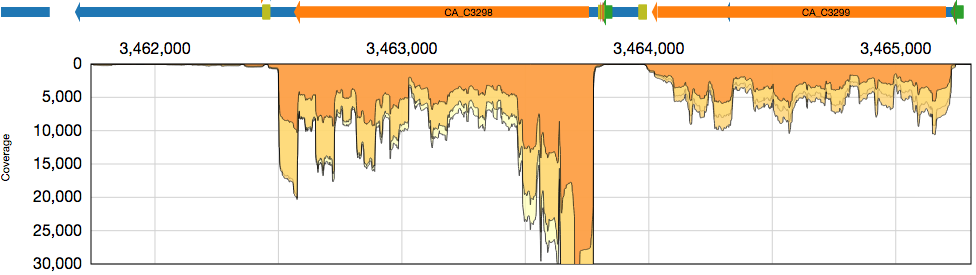
\includegraphics[width=\textwidth,height=1.5in]{images/Assembly/Bdh/Bdh-locus.png}
\subcaption{BdhB(left) and BdhA(right) on the negative strand. Features are colored as above.}\label{fig:4a}}
{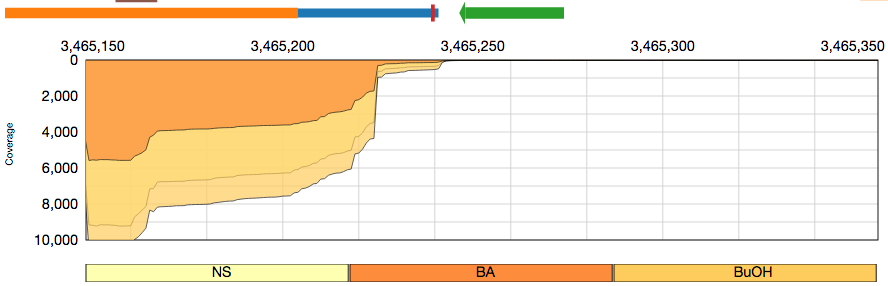
\includegraphics[width=\textwidth,height=1.5in]{images/Assembly/Bdh/BdhA-TSS.png}
\subcaption{BdhA Transcription Initiation Region}\label{fig:4b}}
{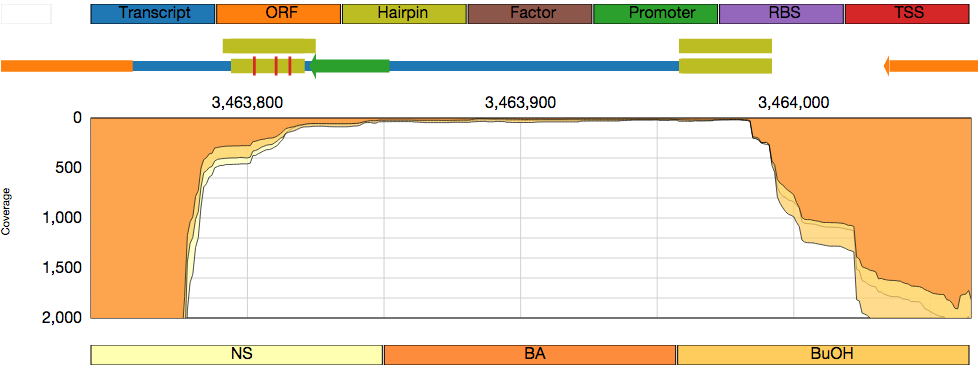
\includegraphics[width=\textwidth,height=1.5in]{images/Assembly/Bdh/BdhB-TSS.png}
\subcaption{BdhB Transcription Initiation Region}\label{fig:4c}}
\caption{Bdh Locus and Transcription Start Sites: \subref{fig:4a}) Both genes in this locus produce distinguishable coverage patterns, and the coverage pattern and assembly agree to a good extent. It is worth noting the trailing 3' UTR after the BdhB ORF and hairpin. Additionally, the BdhA transcript (blue arrow, right) terminates before the end of the ORF and the hairpin. These two regions require minor corrections. \subref{fig:4b}) The BdhA transcript displays a sharp increase in coverage near the transcriptional start site. This data agrees to a good extent with primer extension studies for this gene. \subref{fig:4c}) The BdhB also contains a sharp increase in coverage near the published transcription start site. However, the assembled transcript extends to the nearby terminator. This region also requires minor correction.}
\end{figure}

The GroES and GroEL proteins are heat-shock responsive chaperonins that are required for robust growth at all temperatures. The proteins are highly conserved across all species and are expressed in \textit{C. acetobutylicum} on a 2.15kb transcript, a length consistent with previous studies. These proteins are an integral part of the solvent stress response and the broader stress response systems of this and other bacterial species. A single strong terminator is present at the end of the transcript and promoter motif upstream of the start site was found previously. The observed transcript coordinates are also consistent with previous studies.
\begin{figure}
{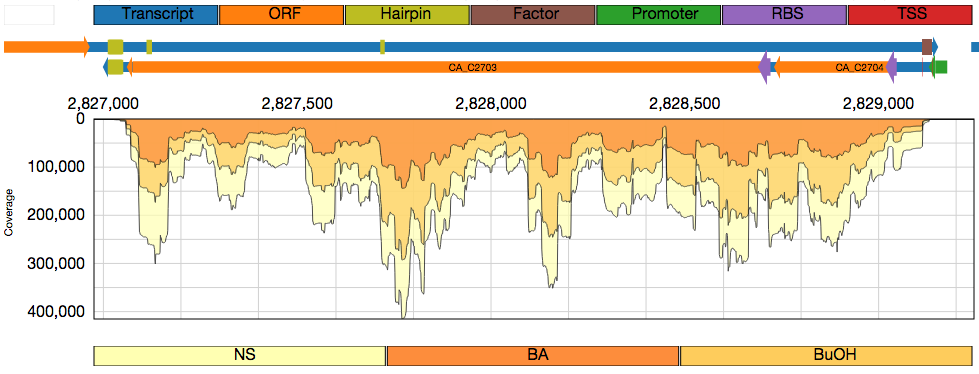
\includegraphics[width=\textwidth,height=1.5in]{images/Assembly/GroESL/GroESL-locus.png}
\subcaption{GroEL (left) and GroES (right) on the negative strand.}\label{fig:5a}}
{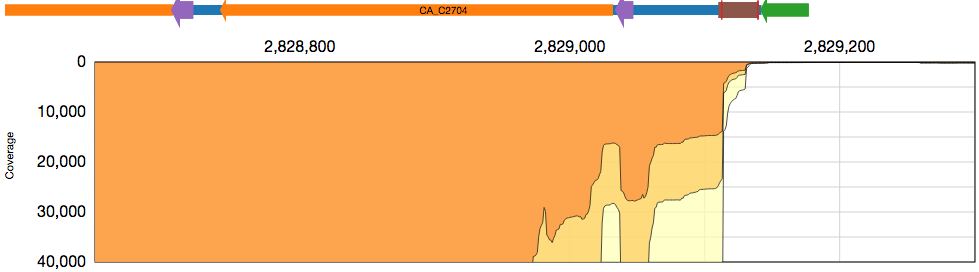
\includegraphics[width=\textwidth,height=1.5in]{images/Assembly/GroESL/GroESL-TSS.png}
\subcaption{GroES/EL operon transcription initiation region}\label{fig:5b}}
\caption{GroES/EL Locus and Transcription Initiation Region: \subref{fig:5a}) GroES and GroEL form an operon that is responsive to heat-shock through a derepression mechanism. The transcript here}
\end{figure}

Spo0A is the master regulator of sporulation and stationary phase phenomena. This protein is thought to ultimately transduce signals into sporulation behavior in a number of sporulating anaerobic firmicutes. In previous studies, Spo0A was shown to be translated from a 0.9kb transcript. Here we observe a slightly longer transcript of ~1.1kb. Unfortunately, the transcript described by this coverage pattern was not detected by state-of-the-art de Bruijn graph assembly. Consequently, this region needs some remediation.

\begin{figure}
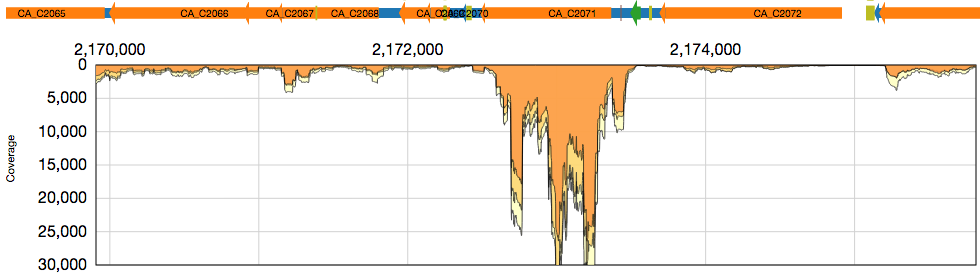
\includegraphics[width=\textwidth,height=1.5in]{images/Assembly/Spo0A/Spo0A-locus.png}
\caption{Spo0A locus. The Spo0A transcript is found in a region of sufficient k-mer complexity and background coverage for the assembled transcript to be fused to signal from neighboring operons. This region clearly requires attention from curation strategies.}
\end{figure}
\subsection{Identify and Attempt to Resolve Remaining Issues}

\subsection{Novel Transcripts}

\subsection{Exploratory Tools}


